\chapter{Attività di Test}
\label{chap:testing}
In questo capitolo vengono descritti i testeffettuati per valutare le prestazioni del sistema sviluppato. Per fare questo genere di test è stato utilizzato \emph{JMeter}: un tool per misurare le prestazioni di un sistema mediante dei test di carico. Durante questi test si confrontano le vecchie API con le nuove, descritte nel Capitolo \ref{chap:implementation}.

\section{Configurazione di JMeter}
\emph{JMeter} è un progetto open source dell'\emph{Apache Foundation}. La vera particolarità di questo software è quella di essere perfettamente configurabile per automatizzare le operazioni di test di carico su macchine remote. Nel nostro caso è stato utilizzato per testare le richieste, mediante le API, al database. Sono stati realizzati due progetti: il primo relativo alle \textit{vecchie API di Zerocoda}, il secondo relativo alle \textit{nuove}, oggetto di questo elaborato. E' stata simulata l'azione concorrenziale di più utenti (thread) che attraverso un dataset di valori pre-inseriti andassero a richiamare le API. Per una corretta interpretazione dei risultati, la configurazione è rimasta la stessa tra i due progetti. È rimasto \textit{invariato il numero di thread}, l'intervallo (in secondi) in cui questi venivano chiamati, e il numero di loop (serie di operazione) eseguito da ogni thread. Le operazioni svolte da ciascun test mirano a simulare l'attività di un utente sul sistema, e in ordine sono:
\begin{enumerate}
    \item Ricerca delle strutture
    \item Ricerca del calendario di una struttura
    \item Ricerca degli slot di un calendario
    \item Prenotazione di un servizio
    \item Cancellazione della prenotazione appena effettuata
\end{enumerate}
I dati inseriti sono stati gestiti attraverso diversi dataset, che a ogni loop fornivano a ciascun thread il parametro da utilizzare nelle richieste. Per evitare errori, in entrambi i progetti si è fatto sì che i thread non prenotassero nello stesso momento lo stesso servizio. La richiesta, una volta effettuata la prenotazione, ne restituiva l'identificativo, che veniva utilizzato dalla richiesta successiva per cancellare la prenotazione dell'utente.

%%%%%%%%%%%%%%%%%%%%%%%%%%%%%%%%%%%%%%%%%%%%%%%%%%%%%%%%%%%%%%%

\section{Risultati Ottenuti}
Di seguito vengono illustrati i grafici realizzati con appositi plugin di JMeter. 
%Il grafico utilizzato prende il nome di \emph{Response Times Graph}. In esso, il tempo di risposta in millisecondi di ogni richiesta (asse delle ordinate) viene calcolato in funzione dell'orario in cui la richiesta è stata effettuata (sull'asse delle ascisse).
Di seguito vengono illustrati i grafici realizzati con appositi plugin di JMeter. Si fa riferimento a due tipologie grafico:
\begin{itemize}
    \item \textbf{Response Time Graph}: il tempo di risposta in millisecondi di ogni richiesta (asse delle ordinate) viene calcolato in funzione dell'orario in cui la richiesta è stata effettuata (asse delle ascisse) 
    \item \textbf{Aggregate Graph}: per ogni richiesta (asse delle ascisse) viene presentata la media dei tempi di risposta in millisecondi (asse delle ordinate)
\end{itemize}

\subsection{Vecchie API}
\begin{figure}
    \centering
    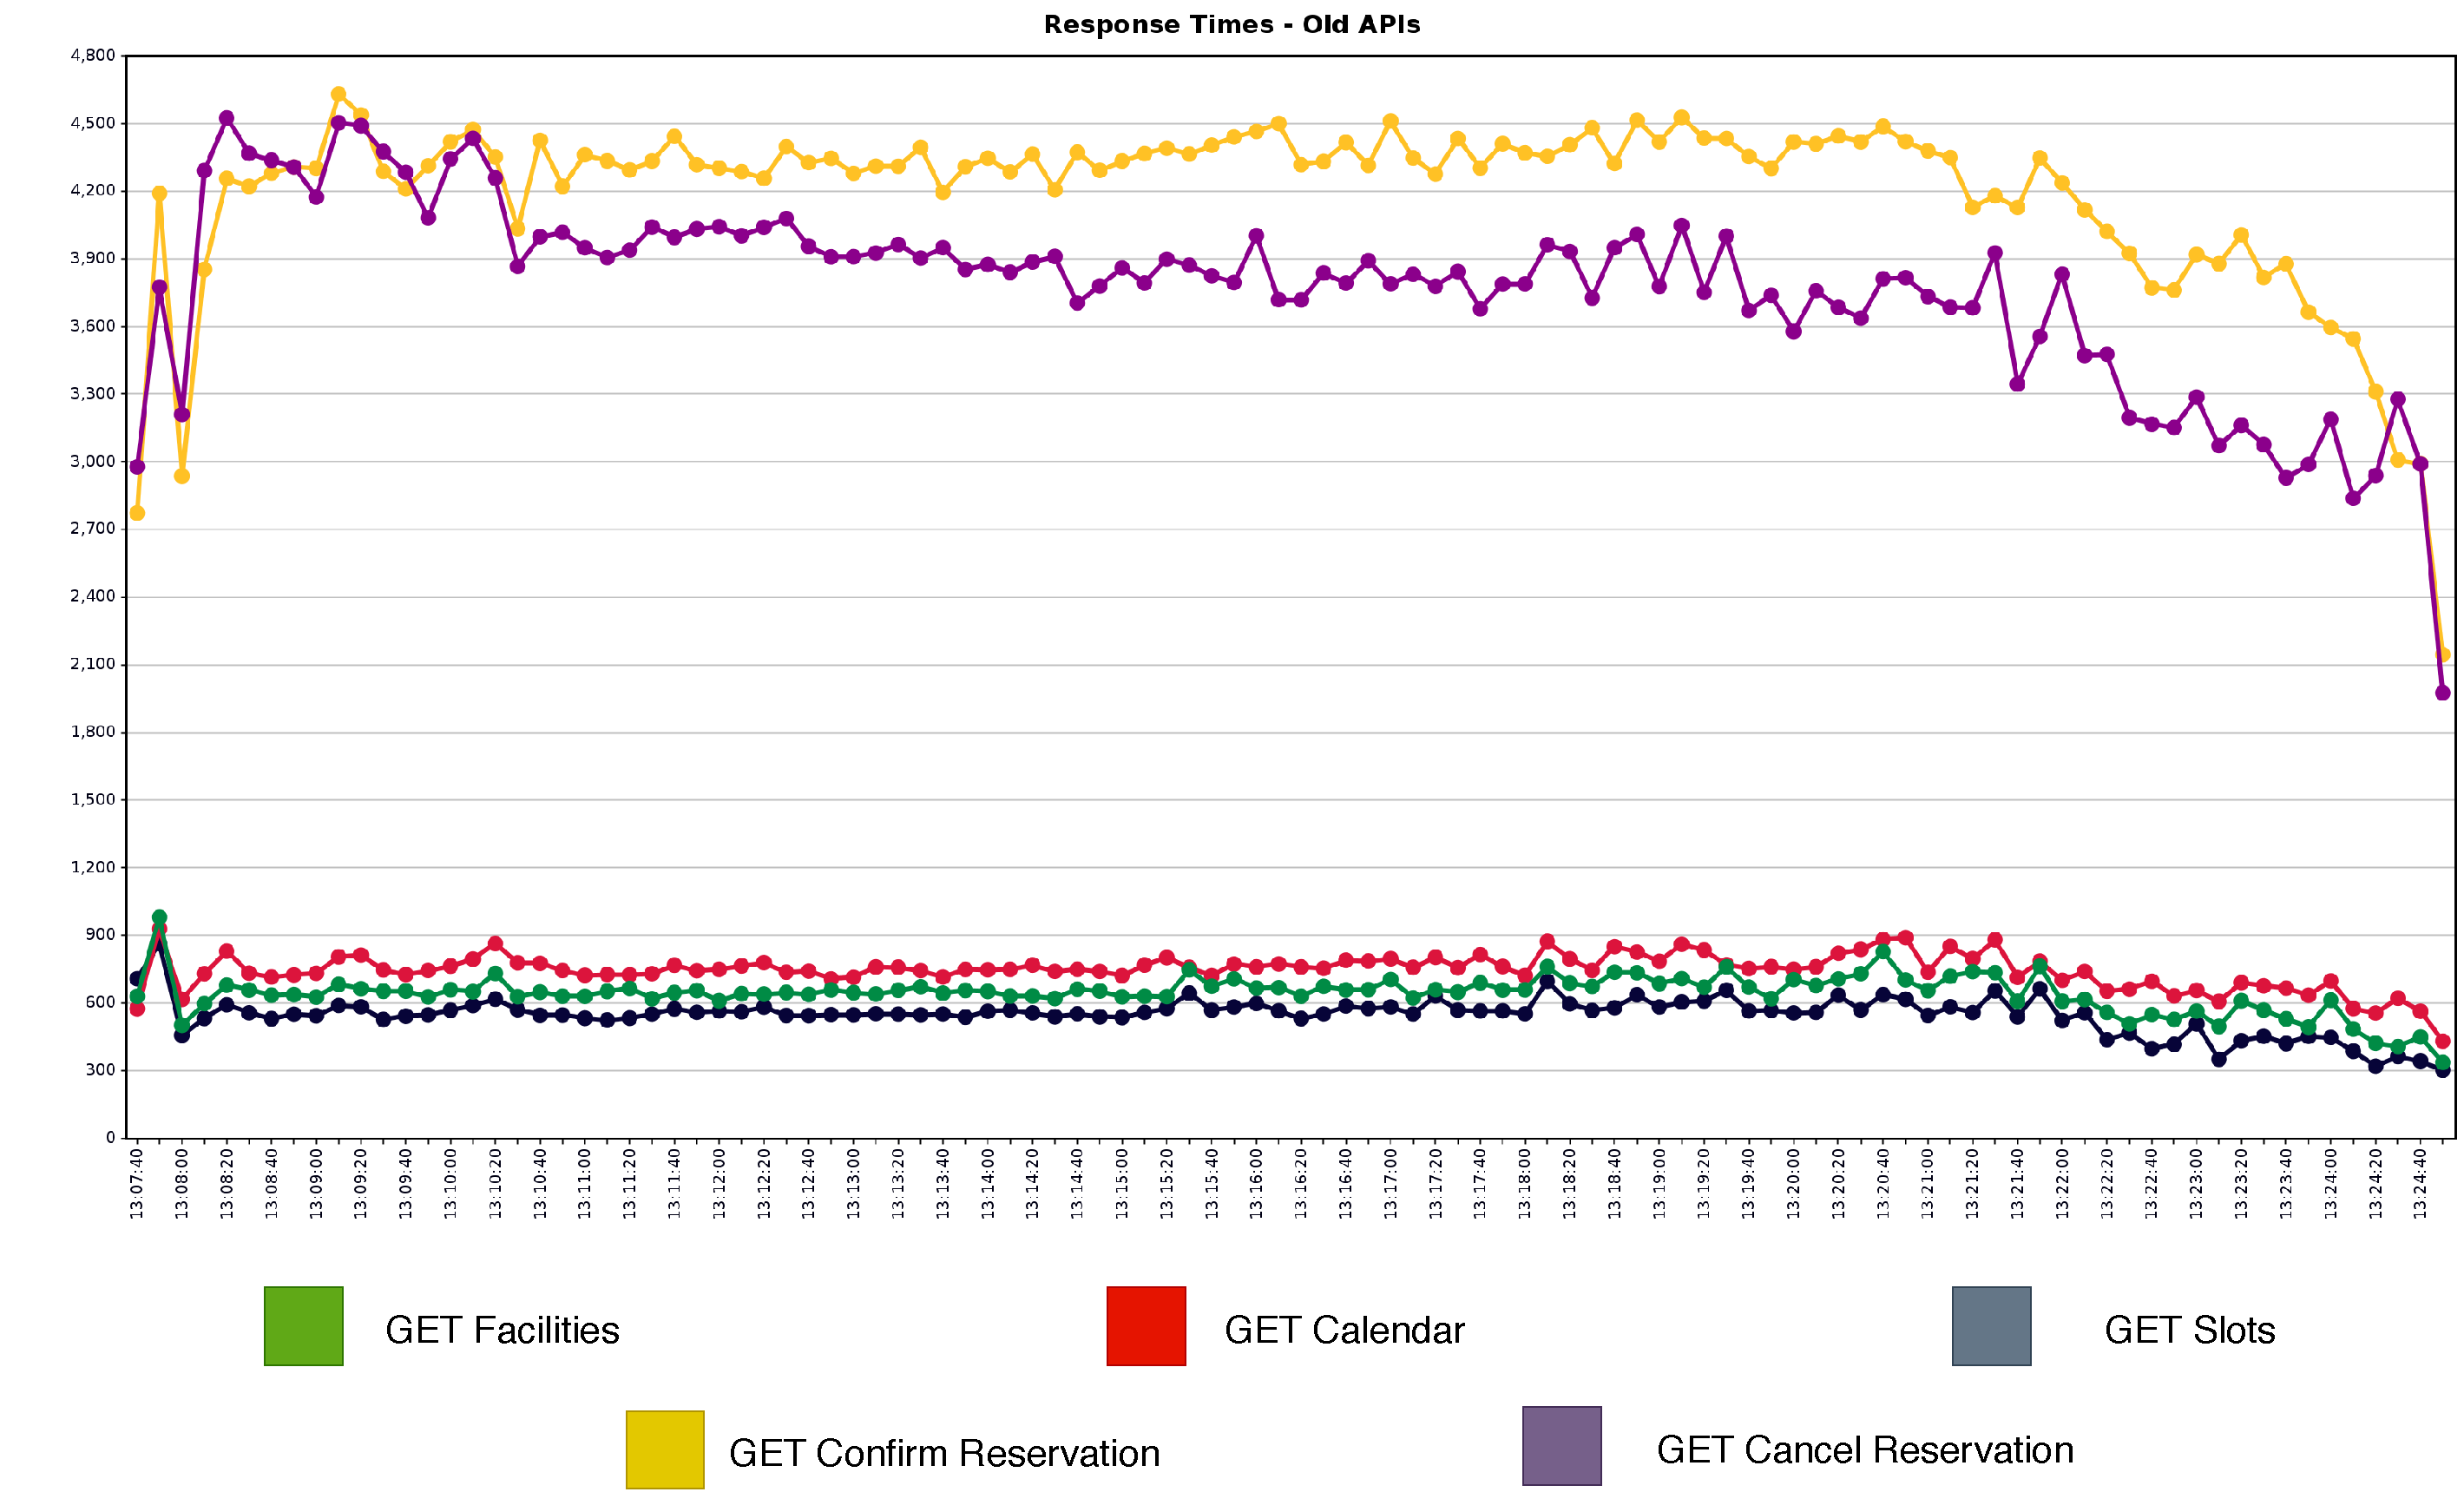
\includegraphics[width=0.90\textwidth]{images/04_1_old_api_response_graph_legend.pdf}
    \caption{Response Times Graph - Old API}
    \label{fig:oldapi100t_response}
\end{figure}
Le API precedenti al refactoring sono messe molto alla prova già con un centinaio di utenti che operano sul sistema (Figura \ref{fig:oldapi100t_response}). Per le operazioni di lettura sul database vengono impiegati circa \emph{800 millisecondi}, mentre il tempo si alza per le operazioni di scrittura, dove una richiesta può impiegare fino a quasi \emph{5000 millisecondi} per restituire una risposta.
%\begin{figure}[H]
%    \centering
%    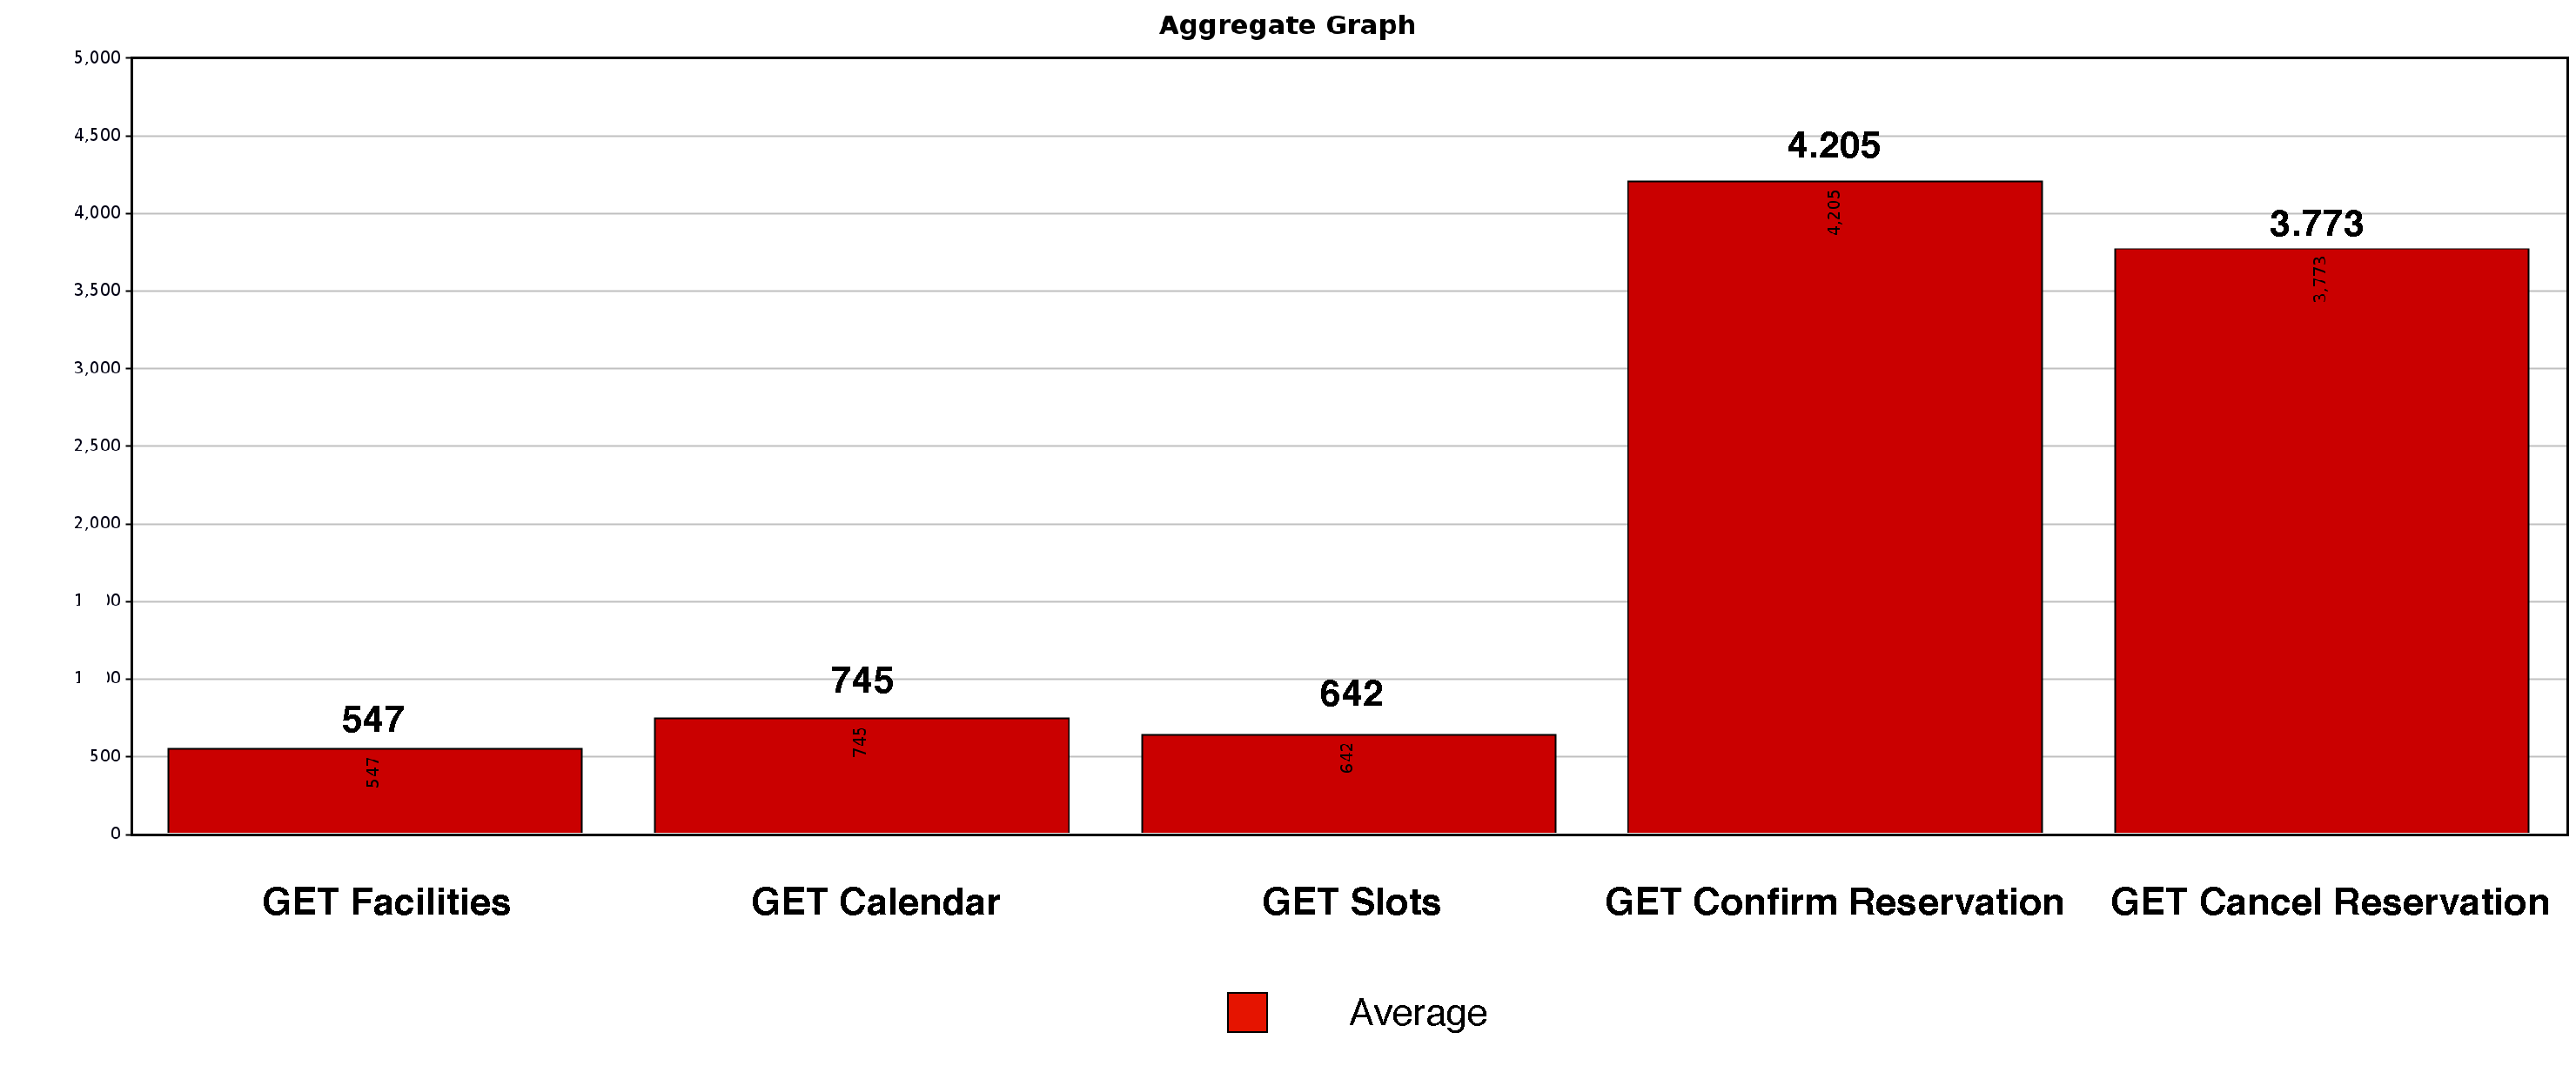
\includegraphics[width=0.80\textwidth]{images/04_2_old_api_aggregate_graph_legend.pdf}
%    \caption{Aggregate Graph - Old API}
%    \label{fig:oldapi100t_aggregate}
%\end{figure}
Nella tabellla mostrata in Figura \ref{fig:oldapi100t_summary} viene mostrata le media (in millisecondi) dei tempi di risposta per ogni richiesta. Anche le richieste più semplici possono impiegare fino a \emph{1000 millisecondi} per l'elaborazione, se il sistema viene messo sotto sforzo.
\begin{figure}[H]
    \begin{table}[H]
        \centering
        \begin{tabular}{ |p{3cm}||p{2cm}|p{2cm}|p{1cm}|p{1cm}|p{2cm}| }
            \hline
            Request & \# Samples & Average  & Min & Max &  Throughput\\
            \hline
            GET Facilities      & 10000    & 547   & 29 & 6625 & 9,65525      \\
            GET Calendar        & 10000    & 745   & 37 & 6546        & 9,65532      \\
            GET Slots        & 10000    & 642   & 31 & 4129        & 9,65546      \\
            GET Conf. Res.        & 10000    & 4205    & 72 & 9978        & 9,65418      \\
            GET Can. Res        & 10000    & 3773    & 96 & 9432        & 9,65309      \\
            TOTAL        & 50000    & 1983    & 29 & 9978        & 48,24383      \\
            \hline
        \end{tabular}
    \end{table}
    \caption{Sommario dei Tempi del Test \textit{[ms]} - Vecchie API}
    \label{fig:oldapi100t_summary}
\end{figure}
Per questo test, così come per il successivo, si è testato uno scenario in cui 100 utenti (threads) eseguono in parallelo le chiamate presentate, per un totale di 100 volte. I \emph{samples} rappresentano il numero di loop in cui è stata eseguita ciascuna richiesta. Si osservino i parametri ottenuti nel \emph{throughput}, e si tengano a mente per un confronto con i corrispettivi valori nelle nuove API.

\subsection{Nuove API}
Le nuove API hanno dato un esito positivo già nel loro tempo totale di esecuzione. I test sono stati eseguiti separatamente, in modo che l'accesso al database da parte di un backend non andasse a influire sulla richiesta di connessione da parte del backend rivale. Il test svolto con le nuove API ha avuto un \emph{tempo di esecuzione quasi 20 volte minore al precedente}. Un risultato straordinario, ma sostenuto da diverse ragioni. In Figura \ref{fig:newapi100t_response} viene presentato il grafico relativo ai tempi di risposta di ciascuna chiamata. I tempi in millisecondi, rispetto al grafico precedente, risultano parecchio ridotti. Anche le chiamate con i metodi POST o DELETE, che vanno ad effettuare delle operazioni di scrittura sul database, hanno comunque dei tempi minori rispetto a una qualsiasi richiesta GET che nelle vecchie API si limitasse a leggere dei valori. Tutte le richieste nel complesso hanno presentato un miglioramento. Se nel primo grafico a seguito di un picco il sistema stabilizzava le risposte su quel tempo, ora a un picco segue un riabbassamento, e \emph{la gestione delle connessioni appare più controllata.} Il picco è limitato a un istante di tempo, e in seguito ad esso il sistema abbassa nuovamente i propri tempi di risposta.
\begin{figure}
    \centering
    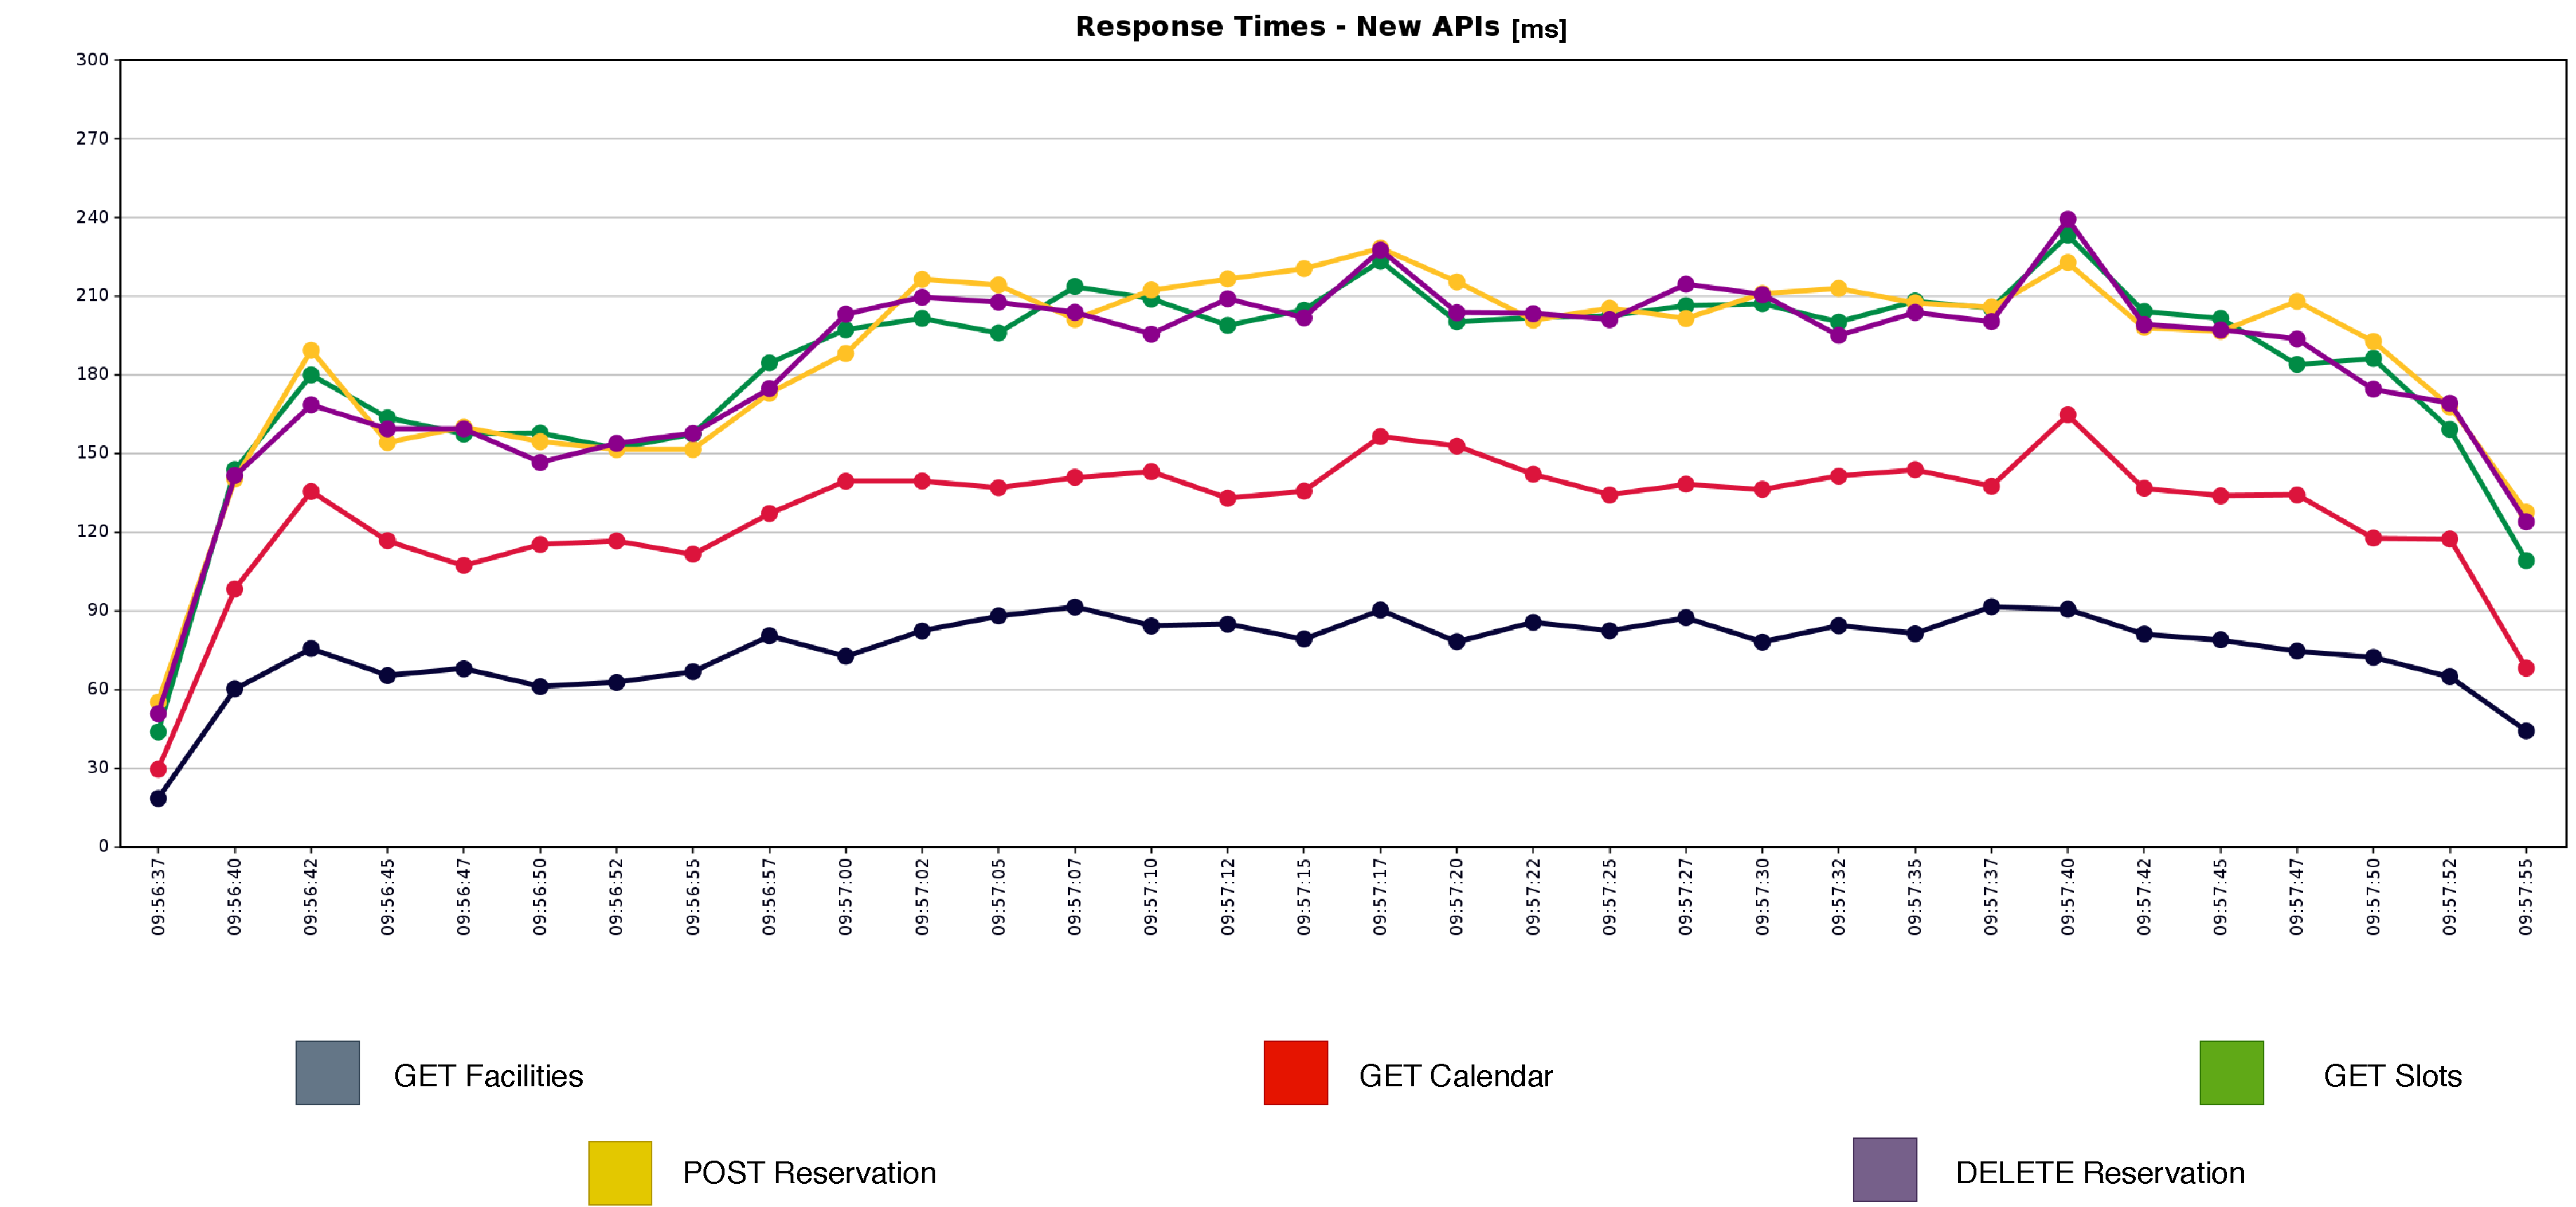
\includegraphics[width=0.90\textwidth]{images/04_2_new_api_response_graph_legend.pdf}
    \caption{Response Times Graph - New API}
    \label{fig:newapi100t_response}
\end{figure}
\begin{figure}[H]
    \begin{table}[H]
        \centering
        \begin{tabular}{ |p{3cm}||p{2cm}|p{2cm}|p{1cm}|p{1cm}|p{2cm}| }
            \hline
            Request & \# Samples & Average  & Min & Max &  Throughput\\
            \hline
            GET Facilities      & 10000    & 89   & 28 & 108 & 100,43993      \\
            GET Calendar        & 10000    & 150   & 49 & 187        & 100,44699      \\
            GET Slots        & 10000    & 223   & 76 & 260        & 100.44295      \\
            POST Reser.        & 10000    & 249    & 98 & 283        & 100,44598      \\
            DELETE Reserv.        & 10000    & 232    & 92 & 311        & 100,45203      \\
            TOTAL        & 50000    & 189    & 28 & 311        & 502,00299      \\
            \hline
        \end{tabular}
    \end{table}
    \caption{Sommario dei Tempi del Test \textit{[ms]} - Vecchie API}
    \label{fig:newapi100t_summary}
\end{figure}
In Figura \ref{fig:newapi100t_summary} vengono mostrati in una tabella i dati relativi al grafico precedente. Le nuove API REST hanno abbassato di molto la media dei tempi di risposta del sistema, \emph{aumentando di diverse unità il throughput}. Questo valore può essere considerato un \emph{indice di misura delle prestazioni del sistema}. Viene misurato in \emph{bit/s} e rappresenta la quantità di informazioni elaborate in un secondo. La differenza tra i due valori è evidente, ma dietro questi numeri c'è da chiedersi: \emph{come fa il sistema dietro le nuove API a garantire dei tempi di risposta tanto più bassi?}

\section{Confronto dei Sistemi}
Vengono illustrati i grafici in Figura \ref{fig:oldapi100t_aggregate} e in Figura \ref{fig:newapi100t_aggregate} rappresentanti la media dei tempi delle due API, a cui si fa riferimento.
\begin{figure}[H]
    \centering
    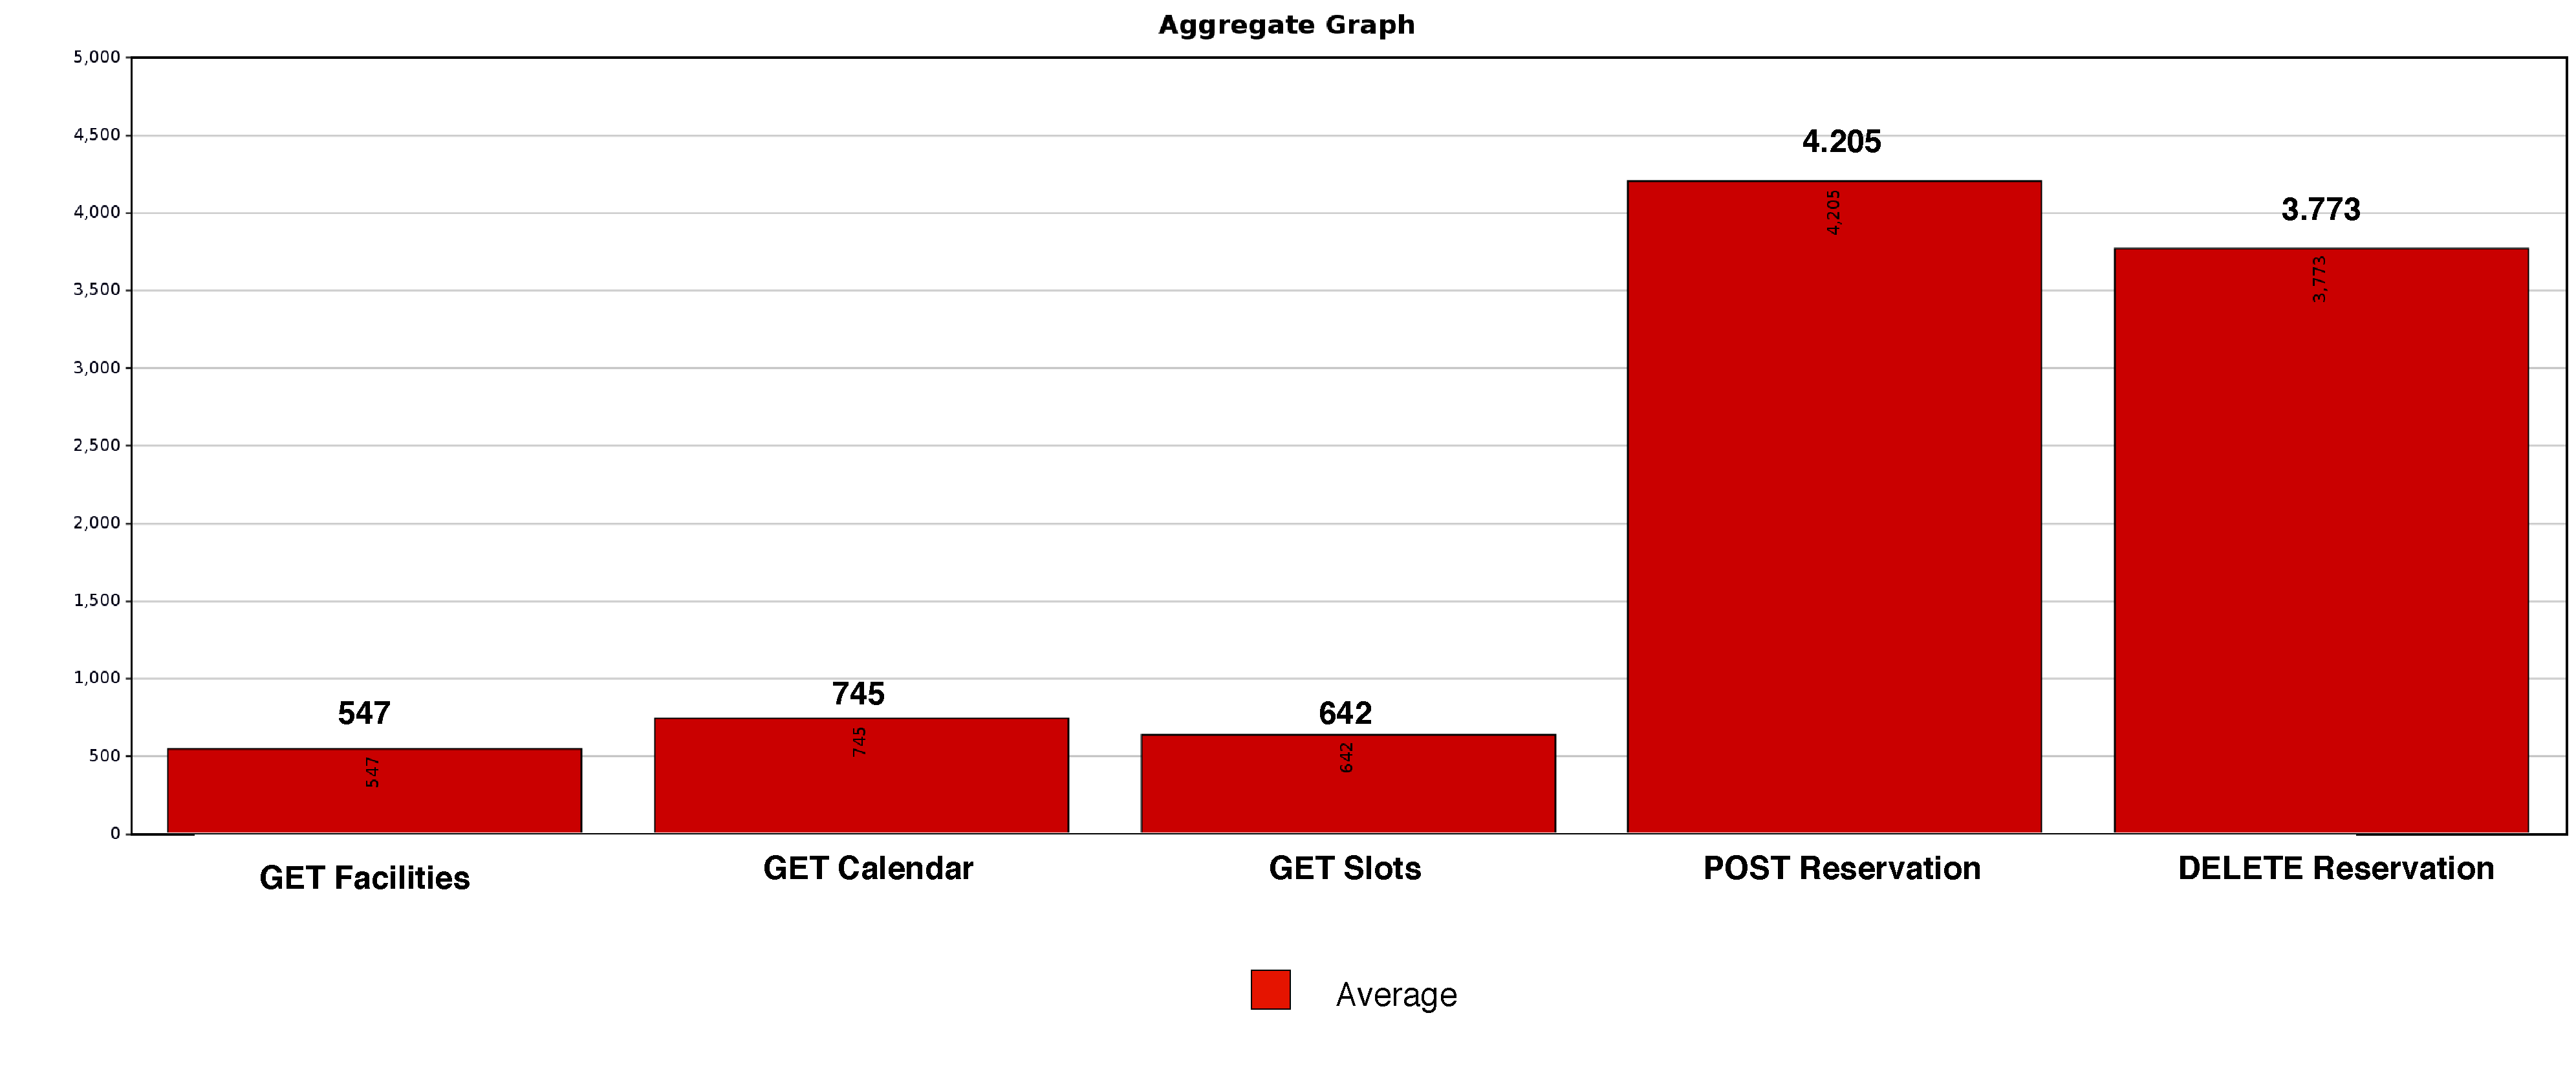
\includegraphics[width=0.95\textwidth]{images/04_3_old_api_aggregate_graph_legend.pdf}
    \caption{Aggregate Graph - Old API}
    \label{fig:oldapi100t_aggregate}
\end{figure}
\begin{figure}[H]
    \centering
    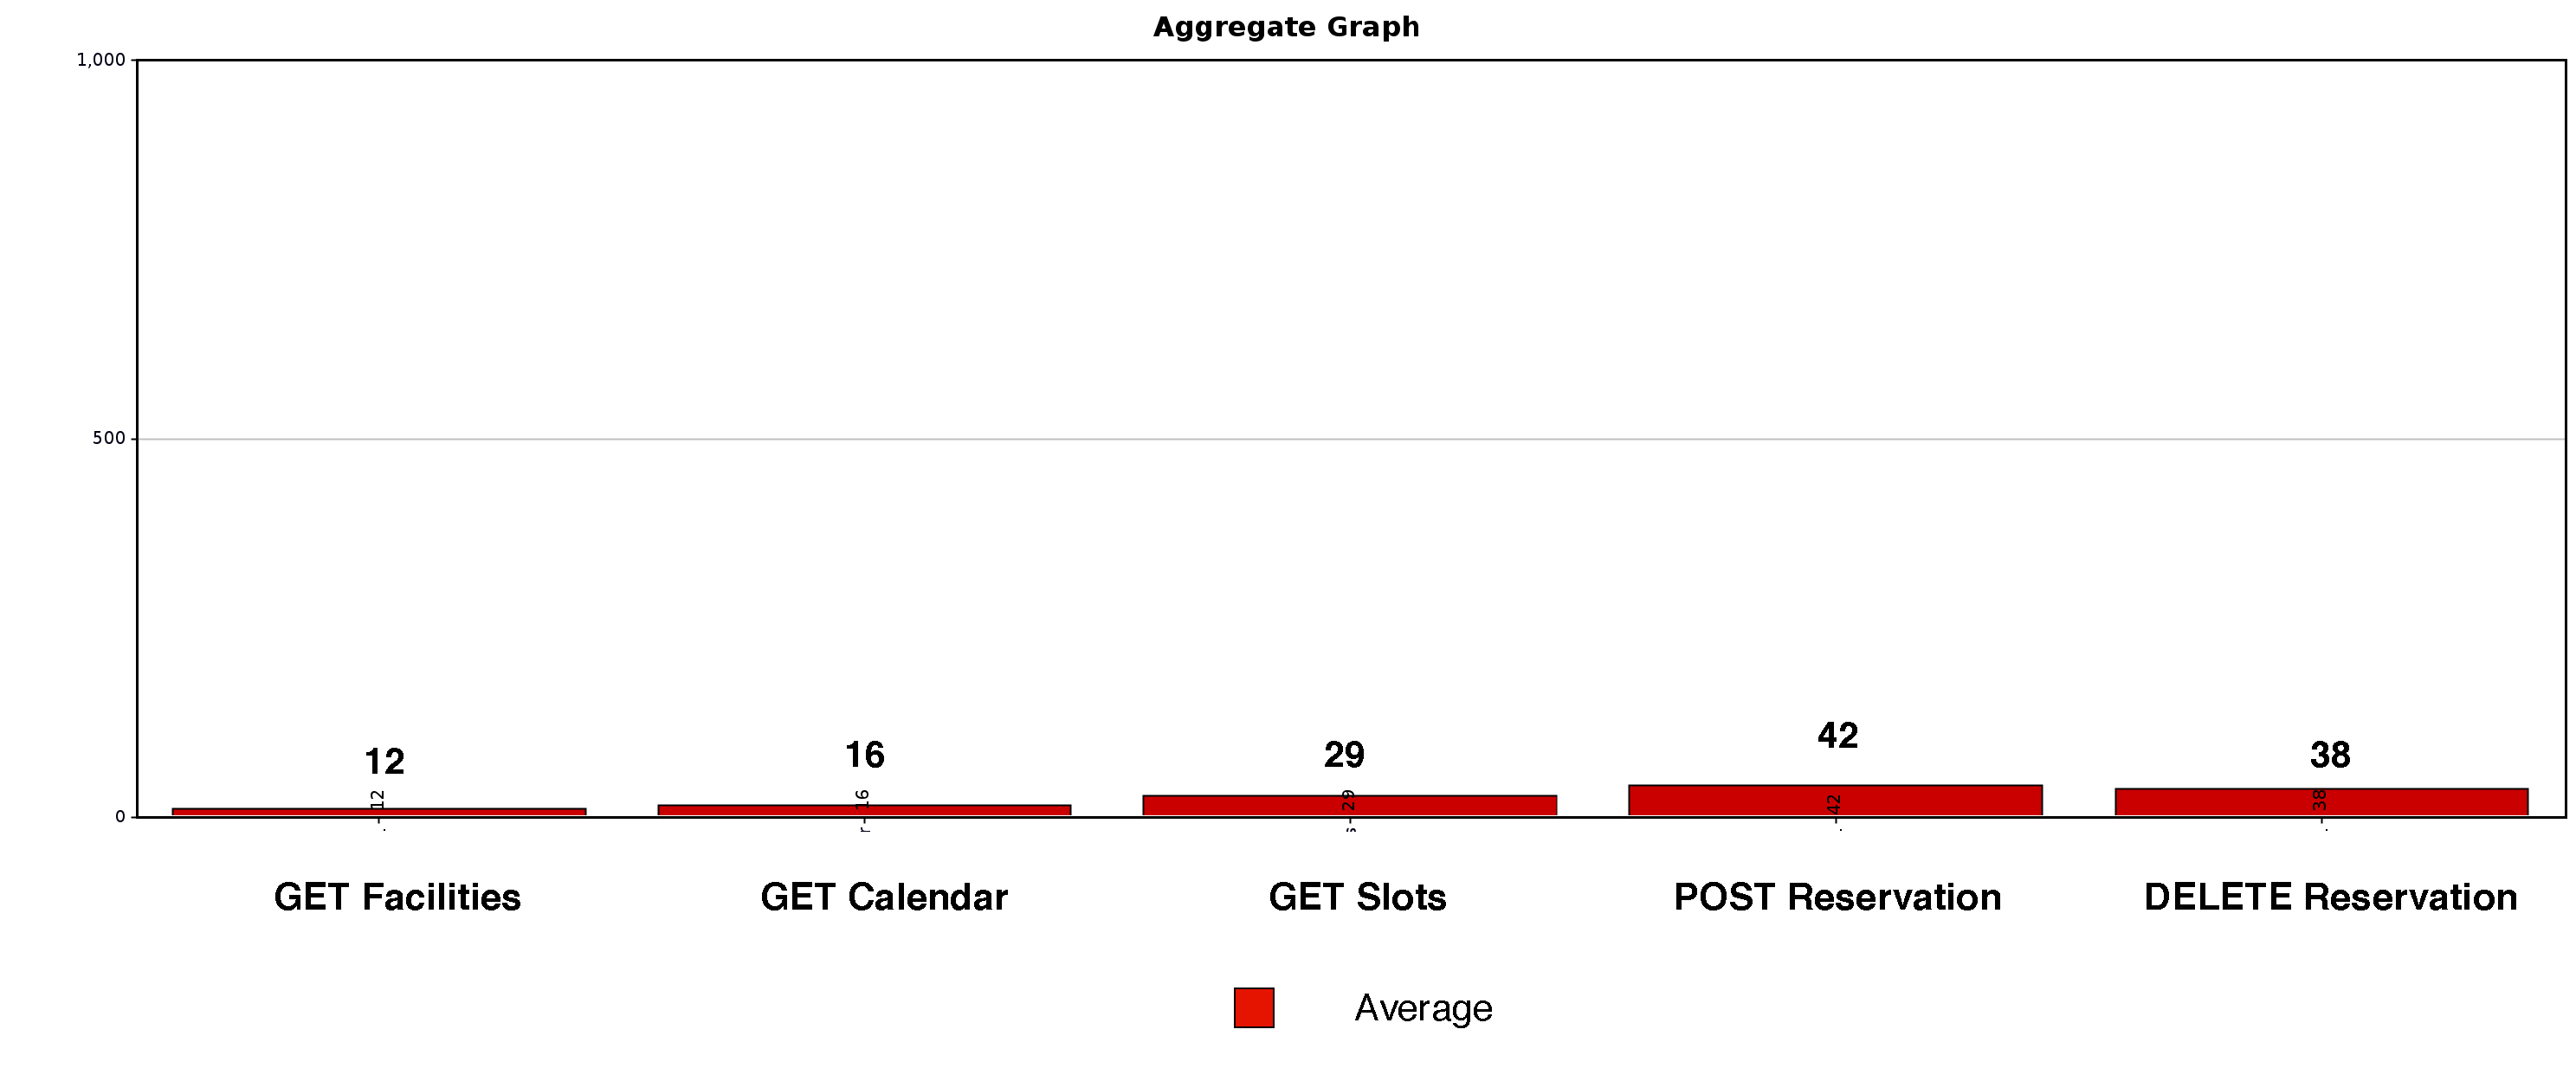
\includegraphics[width=0.95\textwidth]{images/04_4_new_api_aggregate_graph_legend.pdf}
    \caption{Aggregate Graph - New API}
    \label{fig:newapi100t_aggregate}
\end{figure}
La ragione principale degli ottimi risultati ottenuti con la nuova implementazione è banale: l'utilizzo di Java. Il linguaggio rappresenta la prima differenza che salta all'occhio tra i due backend. In PHP, linguaggio usato nella vecchia versione del backend, per ogni richiesta di accesso al database, che fosse questa una richiesta di lettura, scrittura o modifica dei dati, viene creata un'apposita nuova connessione. La connessione viene poi utilizzata dalla chiamata per svolgere l'operazione desiderata, e in seguito chiusa. In Java questa stessa modalità viene migliorata. Ad ogni richiesta è sempre assegnata una connessione, ma spetta al sistema il compito di decidere \emph{a chi} e \emph{quando} assegnarla. Attraverso una \emph{connection pool} le connessioni al database vengono mantenute per velocizzare gli accessi futuri e l'esecuzione dei comandi. In questo modo, ad ogni richiesta non viene più istanziata una nuova connessione, ma a questa ne viene passata una già esistente. Il sistema all'avvio apre un numero ben definito di connessioni al database, e queste vengono assegnate mano a mano alle richieste che ne richiedono l'accesso. In questo modo il backend dietro le nuove REST API riesce sempre a garantire una risposta bassa in termini di millisecondi, il suo tempo di esecuzione risulta ridotto rispetto alla vecchia tecnologia, e il valore di throughput ottenuto risulta nettamente migliore rispetto al precedente.